\chapter{Analytic Framework for Domain-Decomposed Monte Carlo\ }
\label{chap:parallel_theory}
Because we have chosen a domain decomposition strategy in a parallel
environment, this means that communication of these histories must
occur between compute nodes owning neighboring pieces of the global
domain. We wish to characterize this communication not only because
communication is in general expensive, but also because these
nearest-neighbor communication sequences, specifically, have poor
algorithmic strong scaling \cite{gropp_high-performance_2001} in much
the same way as a parallel matrix-vector multiply
operation. Therefore, we desire a framework to provide a simple,
analytic theory based on the properties of the transport system that
will allow for estimates of the domain decomposed behavior of the
Neumann-Ulam method in terms of the amount of information that must be
communicated.

When solving problems where the linear operator is symmetric, a host
of analytic techniques exist based on the eigenvalue spectrum of the
operator that characterize their behavior in the context of
deterministic linear solvers. Using past work, these techniques are
adapted to the domain decomposed Neumann-Ulam method using the
one-speed, two-dimensional neutron diffusion equation and spatial
discretization presented in Appendix~\ref{chap:diffusion_problem} as a
model transport problem. Using the linear system generated by the
discretization of the model problem, we use a spectral analysis to
generate analytic relations for the eigenvalues of the operator based
on system parameters. Using the eigenvalue spectra, we then build
relationships to characterize the transport of stochastic histories in
a decomposed domain and the fraction of histories that leak from a
domain and will therefore have to be communicated. Finally, we compare
these analytic results to numerical experiments conducted with the
model transport problem.

\section{Spectral Analysis }
\label{subsec:spectral_analysis}
The convergence of the Neumann series in
Eq~(\ref{eq:adjoint_neumann_series}) approximated by the Monte Carlo
solver is dependent on the eigenvalues of the iteration matrix. We
will compute these eigenvalues by assuming eigenfunctions of the form
\cite{leveque_finite_2007}:
\begin{equation}
  \Phi_{p,q}(x,y) = e^{2 \pi \imath p x} e^{2 \pi \imath q y}\:,
  \label{eq:eigenfunction_form}
\end{equation}
where different combinations of $p$ and $q$ represent the different
eigenmodes of the solution. As these are valid forms of the solution,
then the action of the linear operator on these eigenfunctions will
yield the eigenvalues of the matrix as they exist on the unit circle
in the complex plane.

For the model problem, we first compute the eigenvalues for the
diffusion operator $\ve{D}$ by applying the operator to the
eigenfunctions and by noting that $x=ih$ and $y=jh$:
\begin{multline}
  \ve{D}\Phi_{p,q}(x,y) = \lambda_{p,q}(\ve{D})
  =\\ -\frac{D}{6h^2}\Big[4 e^{-2 \pi \imath p h} + 4 e^{2 \pi \imath
      p h} + 4 e^{-2 \pi \imath q h} + 4 e^{2 \pi \imath q h} + e^{-2
      \pi \imath p h} e^{-2 \pi \imath q h} \\ + e^{-2 \pi \imath p h}
    e^{2 \pi \imath q h} + e^{2 \pi \imath p h} e^{-2 \pi \imath q h}
    + e^{2 \pi \imath p h} e^{2 \pi \imath q h} - 20\Big] + \Sigma_a
  \:.
  \label{eq:deriv_diff_1}
\end{multline}
Using Euler's formula, we can collapse the exponentials to
trigonometric functions:
\begin{equation}
  \lambda_{p,q}(\ve{D}) = -\frac{D}{6h^2}[ 8 \cos(\pi p h) + 8
    \cos(\pi q h) + 4 \cos(\pi p h) \cos(\pi q h) - 20] + \Sigma_a\:.
  \label{eq:deriv_diff_2}
\end{equation}

As Eq~(\ref{eq:diffusion_eq}) is diagonally dominant, point Jacobi
preconditioning as outlined in
\S~\ref{subsec:stochastic_preconditioning} is sufficient to reduce the
spectral radius of the iteration matrix below unity and therefore
ensure convergence of the Neumann series. Applying this
preconditioner, we are then solving the following diffusion system:
\begin{equation}
  \ve{M}^{-1} \ve{D} \boldsymbol{\phi} = \ve{M}^{-1} \ve{s}\:.
  \label{eq:precond_diffsion}
\end{equation}
The operator $\ve{M}^{-1} \ve{D}$ is merely the original diffusion
operator with each row scaled by the diagonal component. As we have
defined a homogeneous domain, the scaling factor, $\alpha$, is the
same for all rows in the operator and defined as the $\phi_{i,j}$
coefficient from Eq~(\ref{eq:fd_system}):
\begin{equation}
  \alpha = \Bigg[\frac{10 D}{3 h^2} + \Sigma_a\Bigg]^{-1}\:.
  \label{eq:jacobi_scaling}
\end{equation}
Using this coefficient, we then have the following spectrum of
preconditioned eigenvalues:
\begin{equation}
  \lambda_{p,q}(\ve{M}^{-1} \ve{D}) = \alpha \lambda_{p,q}(\ve{D})\:.
  \label{eq:preconditioned_eigenvalues}
\end{equation}

The spectral radius of the iteration matrix is obtained by seeking its
largest eigenvalue. As with the diffusion operator, we can use the
same analysis techniques to find the eigenvalues for the iteration
matrix. We use a few simplifications by noting that if the Jacobi
preconditioned iteration matrix is $\ve{H} = \ve{I} -
\ve{M}^{-1}\ve{D}$, then we expect all terms on the diagonal of the
iteration matrix to be zero such that we have the following stencil:
\begin{multline}
  \ve{H}\boldsymbol{\phi} = \frac{\alpha D}{6h^2}\Big[4 \phi_{i-1,j} +
    4 \phi_{i+1,j} + 4 \phi_{i,j-1} + 4 \phi_{i,j+1}
    +\\ \phi_{i-1,j-1} + \phi_{i-1,j+1} + \phi_{i+1,j-1} +
    \phi_{i+1,j+1}\Big]\:.
  \label{eq:iteration_stencil}
\end{multline}
Inserting the eigenfunctions defined by
Eq~(\ref{eq:eigenfunction_form}) we get:
\begin{multline}
  \lambda_{p,q}(\ve{H}) = \frac{\alpha D}{6h^2}\Big[4 e^{-2 \pi \imath p
      h} + 4 e^{2 \pi \imath p h} + 4 e^{-2 \pi \imath q h} + 4 e^{2
      \pi \imath q h} + e^{-2 \pi \imath p h} e^{-2 \pi \imath q h}
    \\ + e^{-2 \pi \imath p h} e^{2 \pi \imath q q} + e^{2 \pi \imath
      p h} e^{-2 \pi \imath q h} + e^{2 \pi \imath p h} e^{2 \pi
      \imath q h}\Big]\:,
  \label{eq:iteration_deriv}
\end{multline}
which simplifies to:
\begin{equation}
  \lambda_{p,q}(\ve{H}) = \frac{\alpha D}{6h^2}[ 8 \cos(\pi p h) + 8
    \cos(\pi q h) + 4 \cos(\pi p h) \cos(\pi q h)]\:,
  \label{eq:iteration_spectrum}
\end{equation}
giving the eigenvalue spectrum for the Jacobi preconditioned iteration
matrix. We find that the maximum eigenvalue exists when $p=q=0$,
giving the following spectral radius for the Jacobi preconditioned
iteration matrix:
\begin{equation}
  \rho(\ve{H}) = \frac{10 \alpha D}{3 h^2}\:.
  \label{eq:iteration_radius}
\end{equation}

\subsection{Neumann Series Convergence }
\label{subsec:neumann_convergence}
As outlined in \S\ref{sec:mc_preliminaries}, the adjoint Monte Carlo
method is effectively an approximation to a stationary method. In the
adjoint Neumann-Ulam method, $k$ iterations, equivalent to $k$
applications of the iteration matrix, are approximated by a random
walk of average length $k$ to yield the summation in
Eq~(\ref{eq:adjoint_neumann_solution})
\cite{dimov_new_1998,danilov_asymptotic_2000}. This random walk
length, or the number of transitions before the termination of a
history (either by the weight cutoff, absorption, or exiting the
global domain) is therefore approximately the number of stationary
iterations required to converge to the specified tolerance. In the
case of the adjoint Neumann-Ulam method, no such tolerance exists,
however, we have specified a weight cutoff, $W_c$, that determines
when low-weight histories will be prematurely terminated as their
contributions are deemed minute. After $k$ iterations, a stationary
method is terminated as the error has reached some fraction,
$\epsilon$, of the initial error:
\begin{equation}
  ||\ve{e}^{k}||_2 = \epsilon ||\ve{e}^0||_2\:.
  \label{eq:linear_k_iter_norm4}
\end{equation}
Per Eq~(\ref{eq:linear_k_iter_norm3}), we see that this fraction is
equivalent to $\epsilon = \rho(\ve{H})^k$. For the adjoint
Neumann-Ulam method, if we take this fraction to be the weight cutoff,
a measure of how accurately the contributions of a particular history
to the solution are tallied, we then have the following relationship
for $k$:
\begin{equation}
  k = \frac{ \log(W_c) }{ \log( \rho(\ve{H}) ) }\:.
  \label{eq:analytic_k}
\end{equation}
This then gives us a means to estimate the length of the random walks
that will be generated from a particular linear operator based on the
eigenvalues of its iteration matrix (independent of the linear
operator splitting chosen) and based on the weight cutoff parameter
used in the Neumann-Ulam method.

\section{Domain Leakage Approximations }
\label{subsec:domain_leak_approx}
In a domain decomposed situation, not all histories will remain within
the domain they started in and must instead be communicated. This
communication, expected to be expensive, was analyzed by Siegel and
colleagues for idealized, load balanced situations for full nuclear
reactor core Monte Carlo neutral particle simulations
\cite{siegel_analysis_2012}.  To quantify the number of particles
that leak out of the local domain they define a leakage fraction,
$\Lambda$, as:
\begin{equation}
  \Lambda = \frac{average\ \#\ of\ particles\ leaving\ local\ domain}
          {total\ of\ \#\ of\ particles\ starting\ in\ local\ domain}\:.
          \label{eq:leakage_fraction}
\end{equation}
For their studies, Siegel and colleagues assumed that the value of
$\Lambda$ was dependent on the total cross section of the system via
the Wigner rational approximation. Outlined more thoroughly by Hwang's
chapter in \cite{azmy_nuclear_2010}, we will use both the Wigner
rational approximation and the mean chord approximation as a means to
estimate the leakage fraction.

In the case of domain decomposed linear systems, we can use diffusion
theory to estimate the optical thickness of a domain in the
decomposition and the corresponding leakage fraction in terms of
properties of the linear operator and the discretization. To begin we
must first calculate the mean distance a Monte Carlo history will move
in the grid by computing the mean squared distance of its movement
along the chord of length $l$ defined across the domain. After a
single transition a history will have moved a mean squared distance
of:
\begin{equation}
  \langle \bar{r_1^2} \rangle = (n_s h)^2\:,
  \label{eq:step_1_length}
\end{equation}
where $h$ is the size of the discrete grid elements along the chord
and $n_s$ is the number of grid elements a history will move on
average every transition. For our diffusion model problem, $n_s$ would
equate to the expected number of states in the $i$ (or $j$ as the problem is
symmetric) direction that a history will move in a single
transition and is dependent on the stencil used for the
discretization. After $k$ transitions in the random walk, the history
will have moved a mean squared distance of:
\begin{equation}
  \langle \bar{r_k^2} \rangle = k (n_s h)^2\:.
  \label{eq:step_k_length}
\end{equation}
If our chord is of length $l$ and there are $n_i$ grid elements (or
states to which a history may transition) along that chord, then $h =
l / n_i$ giving:
\begin{equation}
  \langle \bar{r_k^2} \rangle = k \Bigg(\frac{n_s l}{n_i}\Bigg)^2\:.
  \label{eq:step_k_length_sub}
\end{equation}
From diffusion theory, we expect the average number of interactions
along the chord to be:
\begin{equation}
  \tau = \frac{l}{2 d \sqrt{\langle \bar{r_k^2} \rangle}}\:,
  \label{eq:optical_thickness_1}
\end{equation}
where $d$ is the dimensionality of the problem and $\sqrt{\langle
  \bar{r_k^2} \rangle}$ is effectively the mean free path of the Monte
Carlo history in the domain. We can readily interpret $\tau$ to be the
\textit{effective optical thickness} of a domain of length
$l$. Inserting Eq~(\ref{eq:step_k_length_sub}) we arrive at:
\begin{equation}
  \tau = \frac{n_i}{2 d n_s \sqrt{k}}\:,
  \label{eq:optical_thickness_2}
\end{equation}
which if expanded with Eq~(\ref{eq:analytic_k}) gives us the final
relation for the effective optical thickness:
\begin{equation}
  \tau = \frac{n_i}{2 d n_s}
  \sqrt{\frac{\log(\rho(\ve{H}))}{\log(W_c)}}\:.
  \label{eq:optical_thickness_3}
\end{equation}

For optically thin domains, we expect that most histories will be
communicated, while optically thick domains will leak the fraction of
histories that did not interact within. Using the optical thickness
defined in Eq~(\ref{eq:optical_thickness_3}), we can then complete the
leakage approximations by defining the bounds of $\tau \rightarrow 0,
\Lambda \rightarrow 1$ and $\tau \rightarrow \infty, \Lambda
\rightarrow \tau^{-1}$.  With these bounds we can then define the
leakage fraction out of a domain for the adjoint Neumann-Ulam method
using the Wigner rational approximation:
\begin{equation}
  \Lambda = \frac{1}{1+\tau}\:,
  \label{eq:wigner_domain_leakage}
\end{equation}
and using the mean-chord approximation:
\begin{equation}
  \Lambda = \frac{1-e^{-\tau}}{\tau}\:.
  \label{eq:mean_chord_domain_leakage}
\end{equation}
Here, the leakage fraction is explicitly bound to the eigenvalues of
the iteration matrix, the size of the domain, the content of the
discretization stencil, and the weight cutoff selected to terminate
low weight histories.

\section{Numerical Experiments }
\label{subsec:numerical_experiments}
To test the relationships developed by the spectral analysis, we form
two simple numerical experiments using the diffusion model problem:
one to measure the length of the random walks as a function of the
iteration matrix eigenvalues, and one to measure the domain leakage
fraction as a function of the iteration matrix eigenvalues and the
discretization properties. Before doing this, we verify our
computation of the spectral radius of the iteration matrix by
numerically computing the largest eigenvalue of the diffusion operator
using an iterative eigenvalue solver. For this verification, a $100
\times 100$ square grid with $h=0.01$, $h=0.1$, and $h=1.0$ and the
absorption cross section varied from 0 to 100 while the scattering
cross section was fixed at unity. Figure~\ref{fig:measured_spec_rad}
gives the measured spectral radius of the iteration matrix and the
computed spectral radius for the preconditioned diffusion operator
using Eq~(\ref{eq:iteration_radius}) as function of the absorption to
scattering ratio $(\Sigma_a / \Sigma_s)$. Excellent agreement was
observed between the analytic and numerical results with all data
points computed within the tolerance of the iterative eigenvalue
solver.
\begin{figure}[t!]
  \begin{spacing}{1.0}
    \begin{center}
      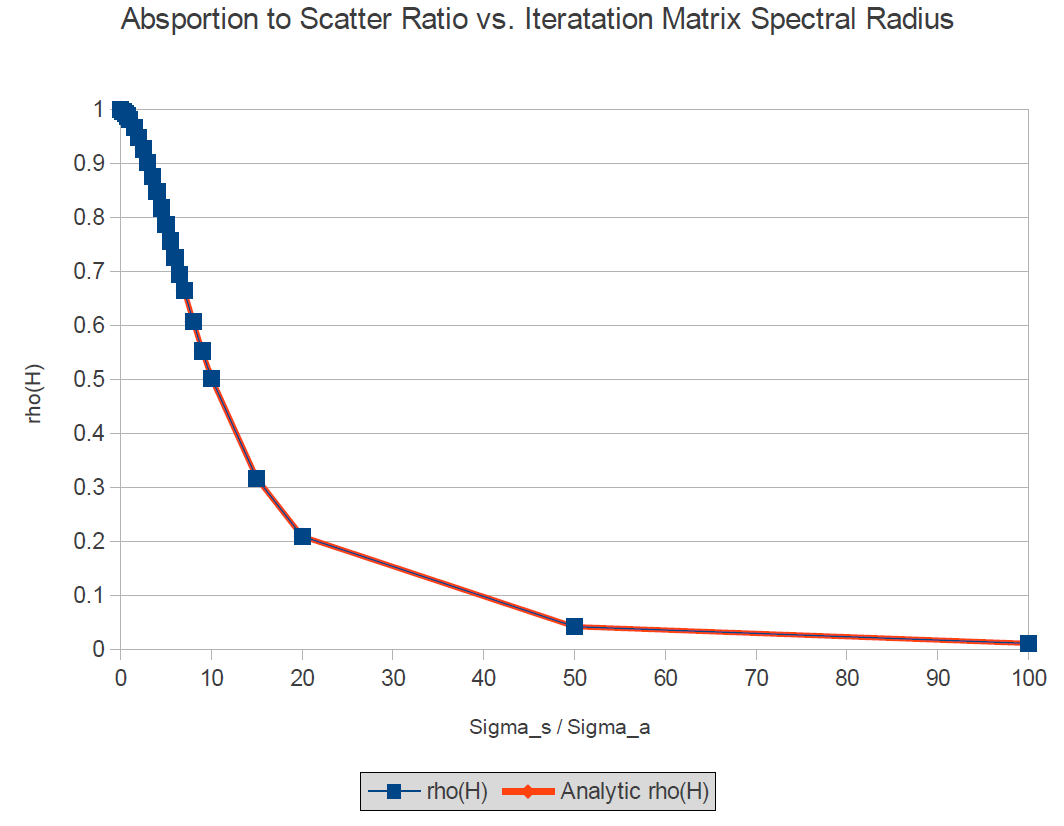
\includegraphics[width=4in,clip]{chapters/parallel_mc/measured_spec_rad.png}
    \end{center}
    \caption{\textbf{Measured and analytic preconditioned diffusion
        operator spectral radius as a function of the absorption cross
        section to scattering cross section ratio.} \textit{Values of
        $h=0.01$, $h=0.1$, and $h=1.0$ were used. The red data was
        computed numerically by an eigensolver while the black dashed
        data was generated by Eq~(\ref{eq:iteration_radius}).}}
    \label{fig:measured_spec_rad}
  \end{spacing}
\end{figure}

\subsection{Random Walk Length }
\label{subsubsec:walk_length}
Next we perform an experiment to measure the length of the random
walks generated by the adjoint Neumann-Ulam solver. To do this, we
again use a $100 \times 100$ square grid with $h=0.1$ and the
absorption cross section varied from 0 to 100 while the scattering
cross section was fixed at unity. Three weight cutoff values of
\sn{1}{-2}, \sn{1}{-4}, and \sn{1}{-8} were used with 10,000 histories
generated by a point source of strength 1 in the center of the
domain. For each of the histories, the number of transitions made was
tallied to provide an effective value of $k$ for each history. This
value was then averaged over all histories to get a measured value of
$k$ for the particular operator. On the left,
Figure~\ref{fig:measured_length} presents these measurements as well
as the analytic result computed by Eq~(\ref{eq:analytic_k}) as a
function of the iteration matrix spectral radius, $\rho(\ve{H})$. On
the right, Figure~\ref{fig:measured_length} gives the relative
difference between the predicted and observed results. We note good
qualitative agreement between the measured and analytic
results. However, we observe a larger relative difference for both
long and short random walks.
\begin{figure}[t!]
  \begin{spacing}{1.0}
    \begin{center}
      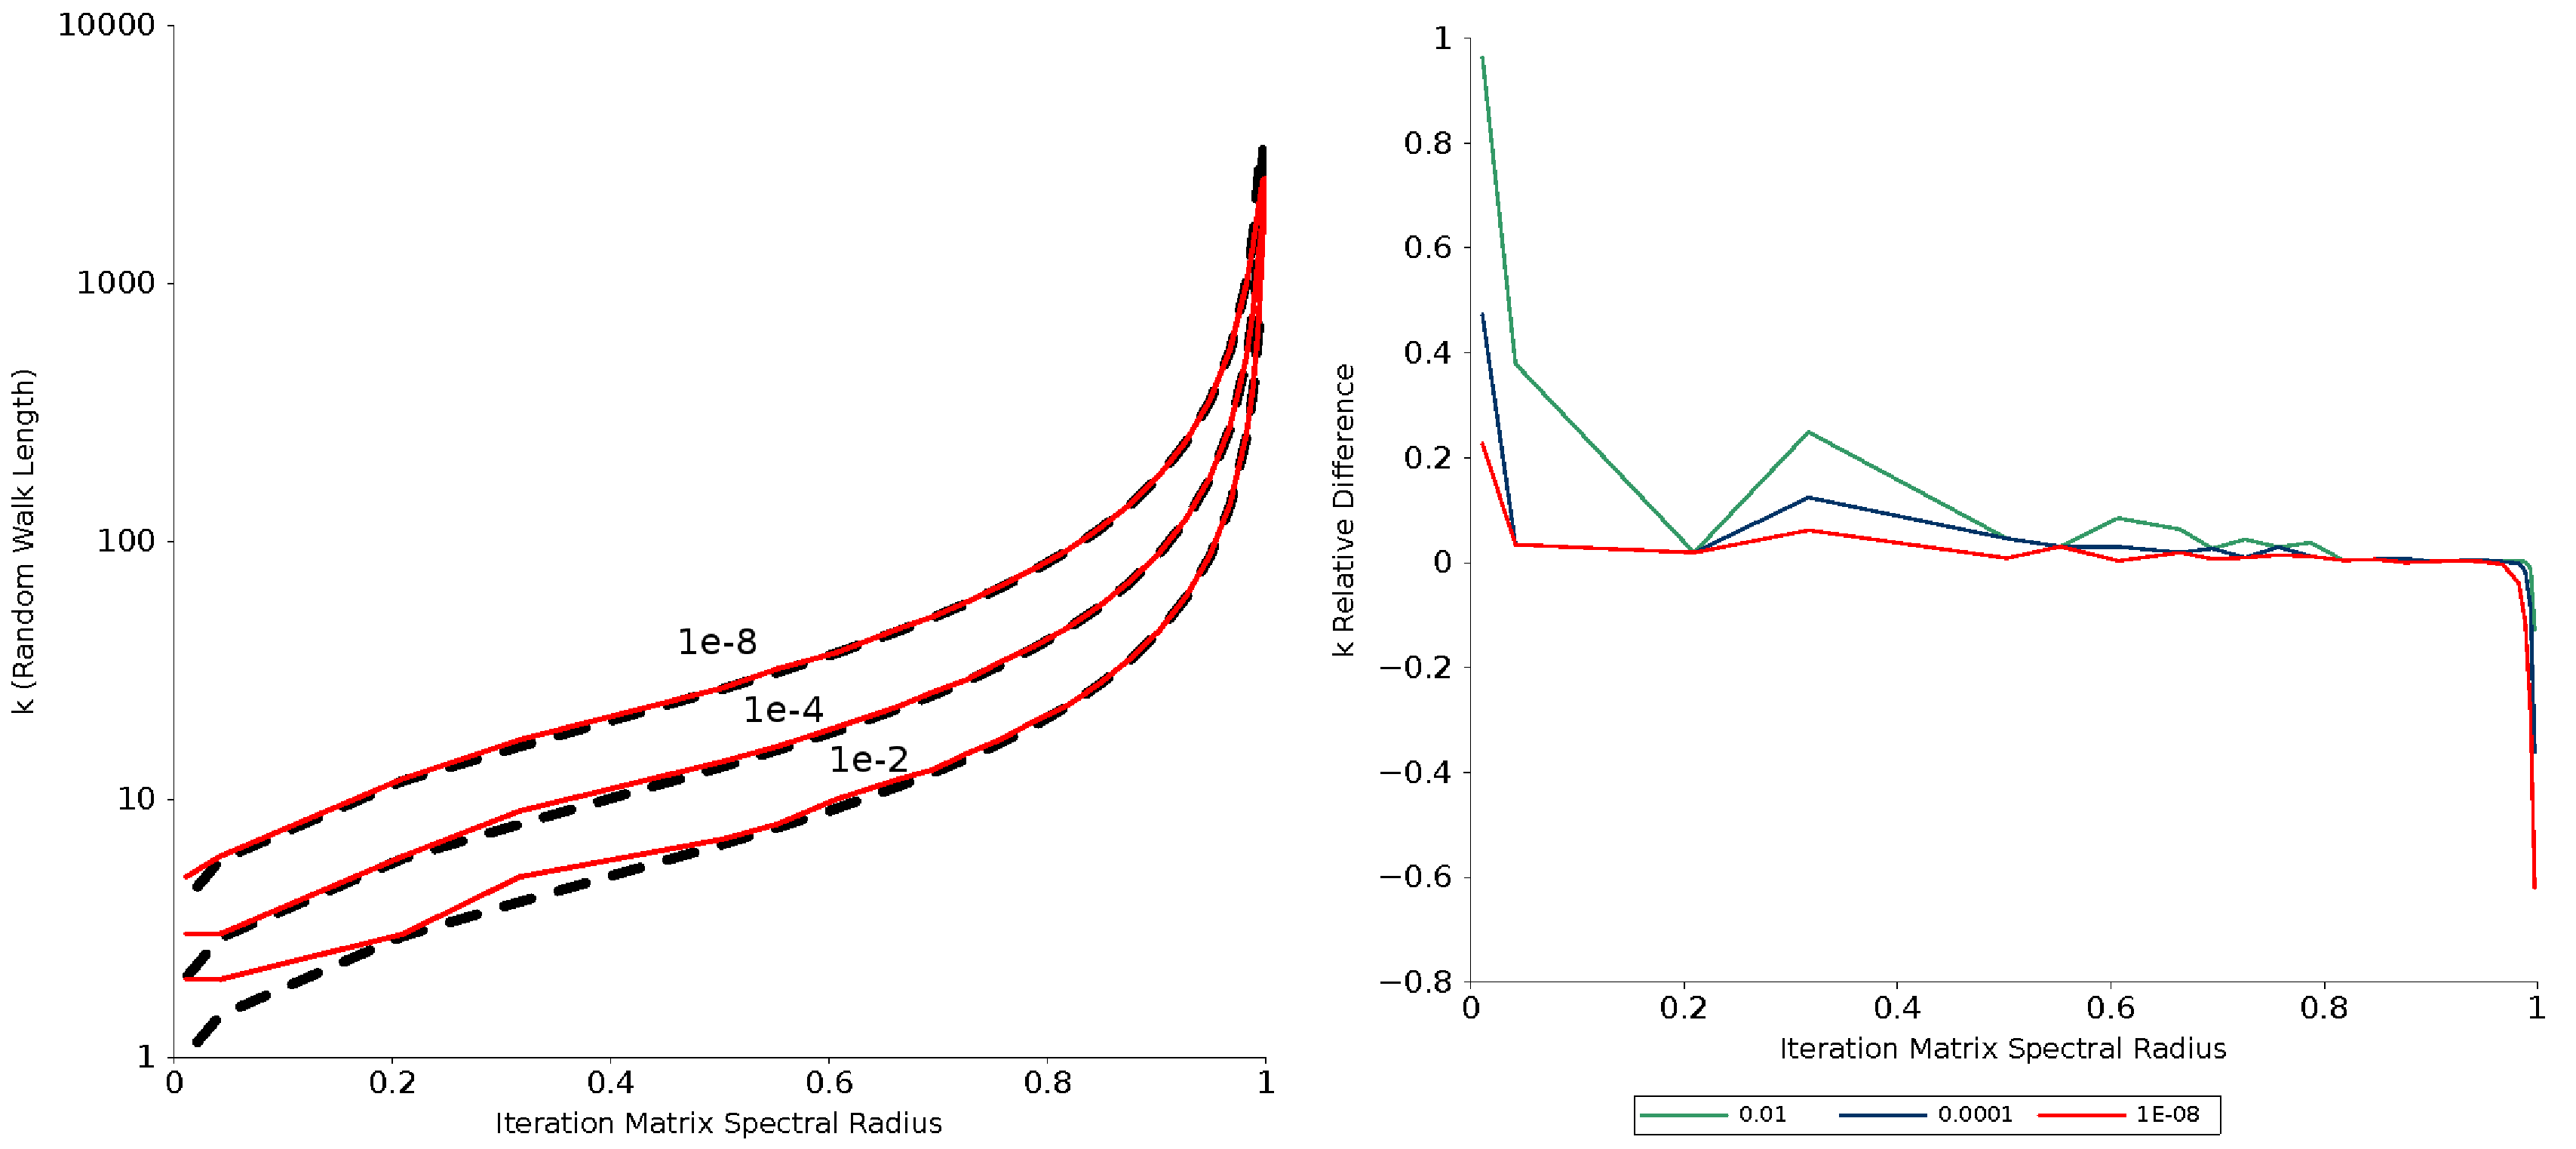
\includegraphics[width=6.0in,clip]{chapters/parallel_mc/measured_length_2.pdf}
    \end{center}
    \caption{\textbf{Measured and analytic random walk length as a
        function of the iteration matrix spectral radius.} \textit{The
        weight cutoff was varied with \sn{1}{-2}, \sn{1}{-4}, and
        \sn{1}{-8}. In the left plot, the red data was computed
        numerically by an adjoint Neumann-Ulam implementation while
        the black dashed data was generated by
        Eq~(\ref{eq:analytic_k}). In the right plot, the relative
        difference between the predicted and measured results is
        presented for each weight cutoff.}}
    \label{fig:measured_length}
  \end{spacing}
\end{figure}

\subsection{Domain Leakage }
\label{subsubsec:domain_leakage}
Finally, we seek to measure the leakage from a domain and assess the
quality of our analytic relation for the optical thickness of a domain
and the associated leakage approximations. For this experiment, a
square grid with $h=0.1$ was decomposed into 9 square domains, 3 in
each cardinal direction with measurements occurring in the central
domain without boundary grid points. For the cross sections, the
absorption cross section was varied from 1 to 100 while the scattering
cross section was set to zero to create a purely absorbing environment
with a weight cutoff of \sn{1}{-4}. The optical thickness of these
domains will then vary as a function of the absorption cross section
if the other parameters are fixed.

To compute the optical thickness, along with the spectral radius as
given by Eq~(\ref{eq:iteration_radius}), we also need the parameters
$n_i$ and $n_s$, which respectively describe the typical domain length
and the average number of states moved along that typical length per
history transition. For our grid above, the domains are varied in size
with $50 \times 50$, $100 \times 100$, and $200 \times 200$ cells
giving $n_i=50$, $n_i=100$, and $n_i=200$ grid points or states along
the typical length of the domain respectively. Looking at the
Laplacian stencil in Eq~(\ref{eq:nine_point_stencil}), we see that all
history transitions will only move a single state in either the $i$ or
$j$ directions due to the symmetry of the problem. Furthermore, if we
choose the $i$ direction, not all states we will transition to will
move the history in that direction. Therefore, we look to the
definition of the iteration matrix in Eq~(\ref{eq:iteration_stencil})
and the definition of the adjoint probability matrix in
Eq~(\ref{eq:adjoint_probability}) to estimate the $n_s$ parameter. For
a particular transition starting at state $(i,j)$, 6 of the 8 possible
new states in the stencil move the history in $i$ direction with
relative coefficients of 4 for moving in the $(\pm i,0)$ direction and
of 1 for moving in the $(\pm i,\pm j)$. These coefficients dictate the
frequency those states are visited relative to the others. For those 6
states we can visit along the typical length, their sum is 12 out of
the total 20 for the coefficients for all possible states with their
ratio giving $n_s = \frac{3}{5}$.

To compute the leakage fraction numerically, \sn{3}{5} histories were
sampled from a uniform source of strength unity over the global
domain. At the start of a stage of histories, the number of histories
starting in the center domain was computed and as the stage
progressed, the number of histories that exited that domain was
tallied with the ratio of the two numbers providing a numerical
measure for the leakage fraction. Figure~\ref{fig:measured_leakage}
gives the domain leakage measurements for the domain in the center of
the global grid as well as the analytic result computed by
Eqs~(\ref{eq:wigner_domain_leakage}) and
(\ref{eq:mean_chord_domain_leakage}) as a function of the iteration
matrix spectral radius.
\begin{figure}[t!]
  \begin{spacing}{1.0}
    \begin{center}
      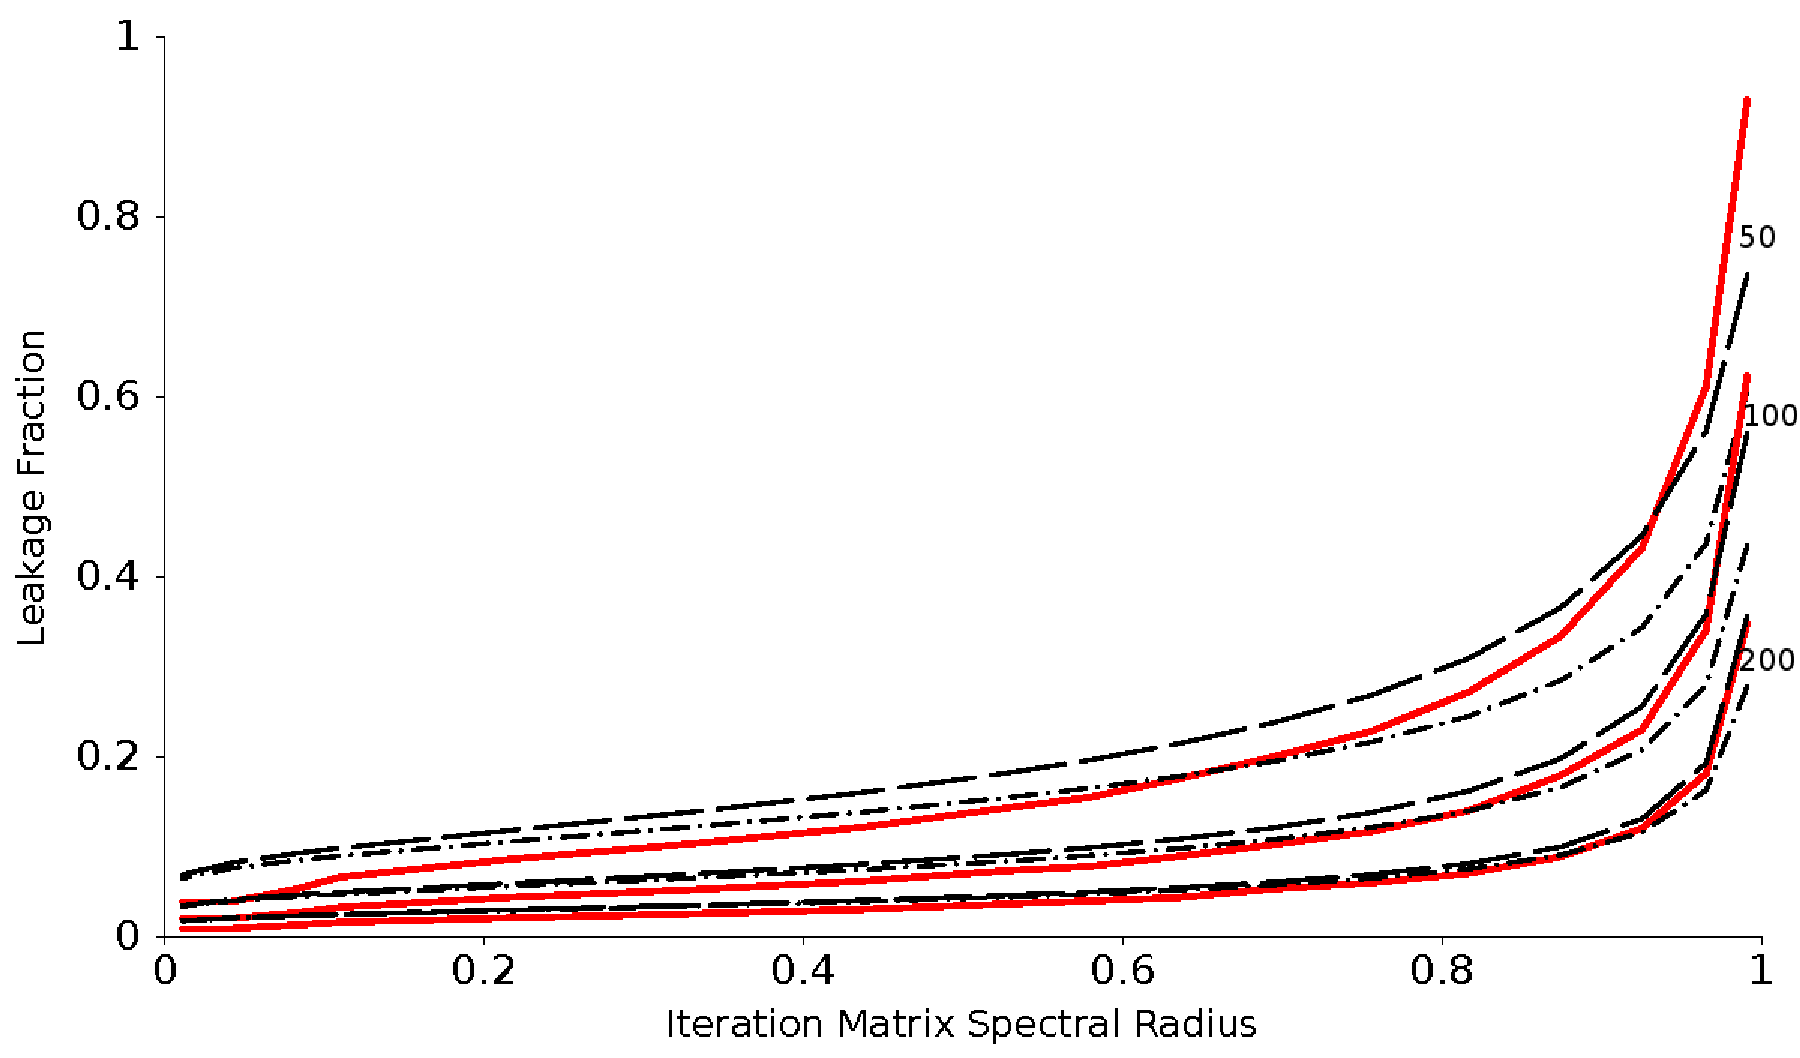
\includegraphics[width=4.75in,clip]{chapters/parallel_mc/leakage_variation_2.pdf}
    \end{center}
    \caption{\textbf{Measured and analytic domain leakage as a
        function of the iteration matrix spectral radius.} \textit{To
        test the behavior with respect to domain size, $n_i=50$,
        $n_i=100$,and $n_i=200$ were used. The red data was computed
        numerically by a domain-decomposed adjoint Neumann-Ulam
        implementation, the black dashed data was generated by
        Eq~(\ref{eq:mean_chord_domain_leakage}) using the mean-chord
        approximation, and the dashed-dotted black data was generated
        by Eq~(\ref{eq:wigner_domain_leakage}) using the Wigner
        rational approximation.}}
    \label{fig:measured_leakage}
  \end{spacing}
\end{figure}
Again, we note good qualitative agreement between the measured and
analytic quantities but we begin to see the limits of the leakage
approximations. 

To compare the quality of the two approximations, the absolute
difference between the computed leakage fraction and that generated by
the Wigner rational and mean chord approximations is plotted in
Figure~\ref{fig:leakage_error} for all domain sizes tested.
\begin{figure}[t!]
  \begin{spacing}{1.0}
    \begin{center}
      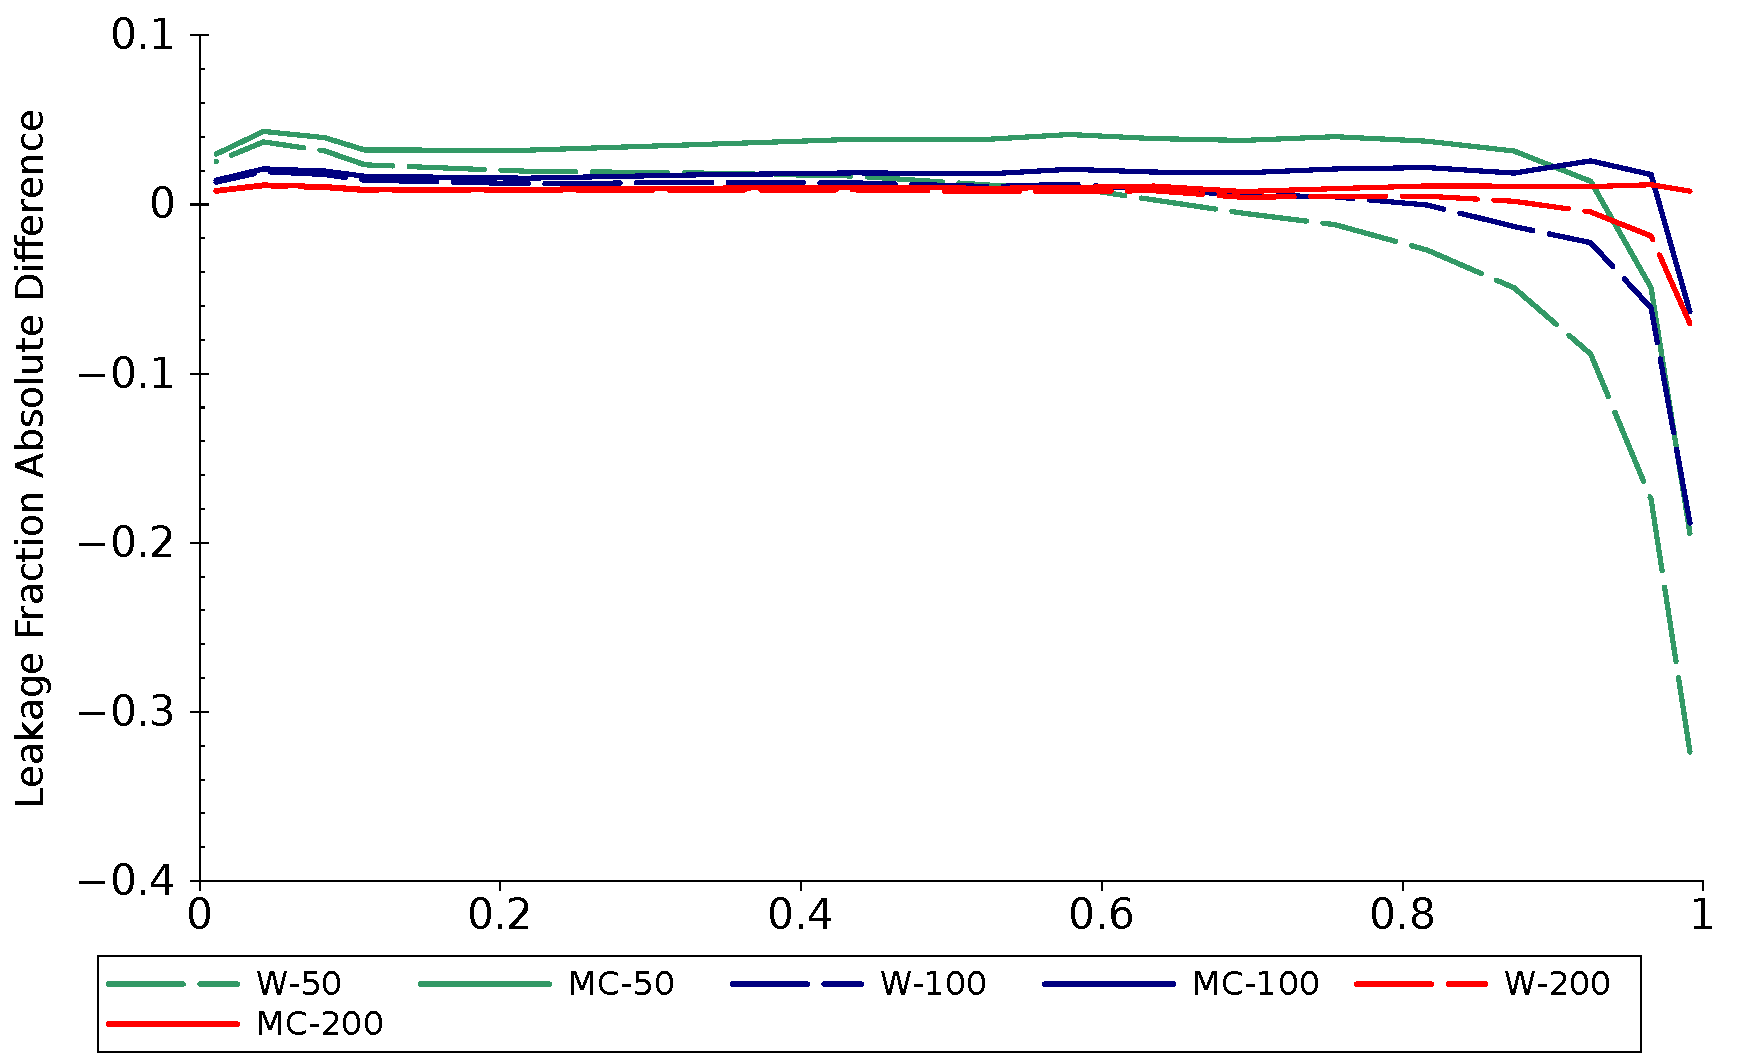
\includegraphics[width=4.75in,clip]{chapters/parallel_mc/leakage_error_2.pdf}
    \end{center}
    \caption{\textbf{Measured and analytic domain leakage absolute
        difference as a function of the iteration matrix spectral radius.}
      \textit{To test the behavior with respect to domain size,
        $n_i=50$ (green), $n_i=100$ (blue), and $n_i=200$ (red) were
        used. The dashed lines represent the difference using the Wigner
        rational approximation while the solid lines represent the
        difference using the mean-chord approximation.}}
    \label{fig:leakage_error}
  \end{spacing}
\end{figure}
From these difference results, the mean chord approximation is shown
to have a lower difference for ill-conditioned systems as compared to
the Wigner approximation while the Wigner approximation produces less
difference for more well-conditioned systems. We also note that for
the optically thick domains, the difference is likely corresponded to
that observed in Figure~\ref{fig:measured_length} for the $k$
parameter while the large relative difference in $k$ for optically
thin domains does not affect the approximation significantly. In
general, the mean chord approximation is a better choice to estimate
the leakage fraction in a domain from the adjoint Neumann-Ulam method
and except for a single data point with $n_i=50$, the mean chord
approximation yielded leakage fractions within an absoulute difference
of 5\% of the measured results. As the domain becomes more optically
thick (with both increasing $n_i$ and decreasing $\rho(\ve{H})$), the
approximations are more accurate.
